\section{Smart Bed}
\begin{figure}[h]
\centering
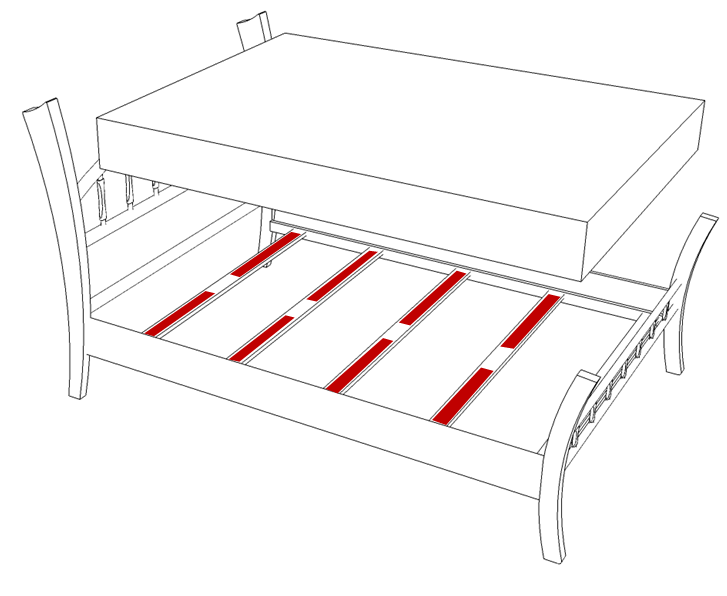
\includegraphics[width=0.7\textwidth]{images/smartbed}
\caption{Smart Bed sketch - flexible plate electrode are attached on spring board}
\label{fig:smartbed_sketch}
\end{figure}
The Smart Bed is a regular bed frame that has been equipped with capacitive proximity sensors in order to determine occupation, posture and sleep phases \cite{braun2012context}\cite{Djakow2013movibed}. A sketch can be seen in Figure \ref{fig:smartbed_sketch}.  The electrodes are comprised of copper foil that is attached to the flexible wooden panels of the slatted frame. This allows the electrodes to be sensitive to both proximity and applied pressure, resulting in a superposed combined sensor value that is considerably higher as opposed to proximity measure on its own. The electrodes are equally distributed, with four being on both sides of the two person bed. The system is able to determine different sitting and lying postures of one or two persons, including less regular lying positions such as diagonal or orthogonal to the long side of the bed. Using an analysis of the movement gathered by variation in the sensor signal the sleep phases can be analyzed, similar to accelerometer-based systems that are popular for smartphones \cite{krejcar2011}.

The Smart Bed can be used for various purposes. A main application is connecting the occupation detection to a home automation system and timer in order to activate ambient lighting if the person is get-ting up in the night, presumably to find the way to the restroom. Accordingly, in a single person household the lights in unoccupied rooms could be turned off in order to conserve energy. In the domain of personal health the Smart Bed is able to give the user a feedback on sleep quality based on the sleep phase measurement performed in the night. Another potential application is to use the acquired pressure distribution as indicator for back-friendly lying positions that may be harmful over a longer period of time \cite{Hamisu2010}.
The occupation and posture detection relies on a simplified body model to approximate the pressure distribution and sensor values to a certain posture \cite{braun2012context}.  
\subsection{Data processing}
\begin{figure}[h]
\centering
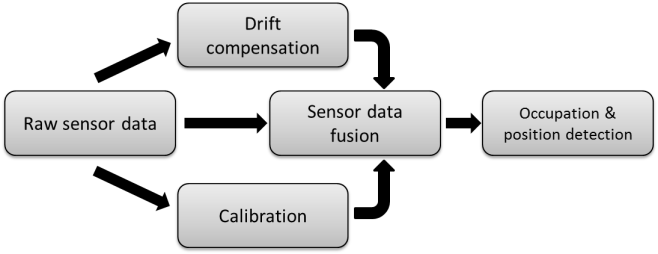
\includegraphics[width=0.7\textwidth]{images/smartbed_proc}
\caption{Data processing components \cite{braun2012context}}
\label{fig:smartbed_proc}
\end{figure}
The different components of the Smart Bed data processing are shown in Figure \ref{fig:smartbed_proc}. Raw sensor data is distributed to three different modules, the calibration which is determining the initial parameters for the sensor data fusion, the drift compensation that alters those parameters according to long term trends and finally the sensor data fusion module that processes the data and does feed it to the occupation \& position detection. Calibration and drift compensation follow the previously presented model \cite{braun2012context}. 
\begin{figure}[h]
\centering
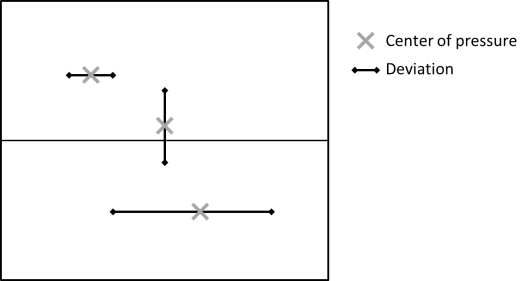
\includegraphics[width=0.7\textwidth]{images/smartbed_cog}
\caption{Calculating centers of pressures and deviation \cite{braun2012context}}
\label{fig:smartbed_cog}
\end{figure}
Occupation and position detection is performed by dividing the two person bed into left and right and individually calculating for each side the total sensor values, assumed center of pressure using weighted average and the standard deviation (Figure \ref{fig:smartbed_cog}). The same calculation is done between the two sides to distinguish where is activity or if one person is lying diagonally.
Using these six intermediate values we can now map various poses. If all activity is on one side and the horizontal deviation is low, we can assume that one person is sitting. We can additionally use the intermediate values to calculate more information, e.g. the exact location a person is sitting at. 
The data processing for the sleep phase recognition is based on detecting the sensor data variations in order to analyze movement. Discriminating between sleep phases using movement is a common approach that has been used in the past \cite{salmi86}. Using a sparse set of sensors it is possible to detect movement by comparing subsequent sensor readings and associate it to different sleep phases using different activity profiles. The system is based on the same prototype as the posture recognition system \cite{Djakow2013movibed}. 
\subsection{Evaluation}
\begin{figure}[h]
\centering
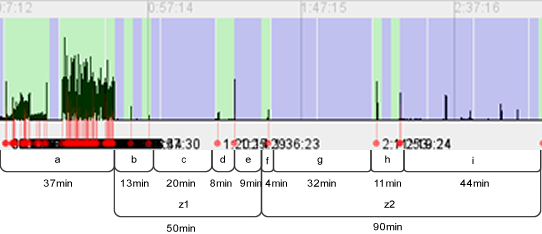
\includegraphics[width=0.9\textwidth]{images/smartbed_sleepphase}
\caption{Sleep movement data over three hours in one night \cite{Djakow2013movibed}}
\label{fig:smartbed_sleepphase}
\end{figure}
The Smart Bed posture recognition is able to successfully distinguish eight typical sitting and lying states. Using adaptation of the intermediate values it is possible to fit the state to an actual position on the bed, e.g. a \emph{person sitting on the right side of the bed} state can be modified to any location on that specific side of the bed. 
Regarding the detection of sleep phases there has been an evaluation and benchmarking of three nights \cite{Djakow2013movibed}. The Smart Bed was able to achieve a comparable performance to smartphone applications that detect sleep phases based on accelerometers. Figure \ref{fig:smartbed_sleepphase} gives an example of movement recordings using the capacitive proximity sensors over one night. The activities are grouped into distinct chunks that are later associated to the sleep phases. Currently breathing rate detection is added to the Smart Bed that can be used to improve the sleep phase detection and also can potentially detect anomalies that may be indicative of a certain health risk.
